%%%%%%%%%%%%%%%%%%%%%%%%%%%%%%%%%%%%%%%%%
% Chair of Cyber-Physical-Systems
% Univ.-Prof. Dr. Elmar Rueckert
% Montanuniversität Leoben, Austria
% Latest Update: Feb. 2022
%
% Disclaimer: The materials and source code are for personal use only. The material is intended for educational purposes only. Reproduction of the material for any purposes other than what is intended is prohibited. The content is to be used for educational and non-commercial purposes only and is not to be changed, altered, or used for any commercial endeavor without the express written permission of Professor Rueckert. 
% 
% Original Version by Frits Wenneker, 28/2/17,  License: CC BY-NC-SA 3.0 (http://creativecommons.org/licenses/by-nc-sa/3.0/)
%%%%%%%%%%%%%%%%%%%%%%%%%%%%%%%%%%%%%%%%%

%----------------------------------------------------------------------------------------
%	PACKAGES AND OTHER DOCUMENT CONFIGURATIONS
%----------------------------------------------------------------------------------------

\documentclass[10pt, a4paper, twocolumn]{article} % 10pt font size (11 and 12 also possible), A4 paper (letterpaper for US letter) and two column layout (remove for one column)

\input{structure.tex} % Specifies the document structure and loads requires packages

%----------------------------------------------------------------------------------------
%	ARTICLE INFORMATION
%----------------------------------------------------------------------------------------

\title{Assignment I: Latex and Python Basics} % The article title

\author{
	\coursetitle{Exercises in Machine Learning (190.013), SS2022}
	\authorstyle{Joe Mann\textsuperscript{1} and Anne Frank\textsuperscript{2}} % Authors
	\newline\newline % Space before institutions
	\textsuperscript{1}\textit{joe.mann@unileoben.ac.at}, \institution{Montanuniversität Leoben, Austria}\\ % Institution 1
	\textsuperscript{2}\textit{anne.frank@unileoben.ac.at}, \institution{Montanuniversität Leoben, Austria}\\ % Institution 1
	\newline\submissiondate{\today} % Add a date here
}

% Example of a one line author/institution relationship
%\author{\newauthor{John Marston} \newinstitution{Universidad Nacional Autónoma de México, Mexico City, Mexico}}


%----------------------------------------------------------------------------------------

\begin{document}
\input{python_code.tex} % To print Python code

\maketitle % Print the title

\thispagestyle{firstpage} % Apply the page style for the first page (no headers and footers)

%----------------------------------------------------------------------------------------
%	ABSTRACT
%----------------------------------------------------------------------------------------

\lettrineabstract{This latex template provides some instructions on how to format your assignment report. Feel free to use your favorite latex editor. Follow the structure below if it suits your needs.}

%----------------------------------------------------------------------------------------
%	REPORT CONTENTS
%----------------------------------------------------------------------------------------

\section{Introduction}
A short introduction to the problem.

You may want to list your contributions using the command \textit{itemize}.

\begin{itemize}
	\item First item in a list 
	\item Second item in a list 
	\item Third item in a list
\end{itemize}

\section{Methods}
Something about the used methods.

Define your equations using the \textit{align} environment. or using \textit{eqnarray}. 

\begin{align}
	A = 
	\begin{bmatrix}
		A_{11} & A_{21} \\
		A_{21} & A_{22}
	\end{bmatrix}
\end{align}

\begin{eqnarray}\label{eq:linRegModel}
y &=& w_1 + w_2 x_1 + w_3 x_2 + \dots + w_{D+1} x_D, \nonumber \\
y &=&  \bm x^T \bm w.
\end{eqnarray}

\subsection{Referencing related work}

You may want to use \textit{Google Scholar} to find related scientific publications. Download the bib files and add the entries to the file \textit{literature.bib}. Below are some examples of how to refer to related works. 

The reader should get a copy of Bishop's book on pattern recognition and machine learning \citep{bishop2006pattern} from our library. Also highly recommended are the books of Murphy and Williams \etal \citep{murphy2012machine, williams2006gaussian}.  Also make sure to refer to all artwork like Figure \ref{fig:pythonPlotOne}.

\subsection{You may add more structure to your report}

Your assignment report should comply with the following structure. Feel free to add latex structure elements like 
\begin{verbatim}
\paragraph*{...}, \subsubsection*{...} \end{verbatim}
\begin{verbatim}
\begin{itemize}..., \begin{enumerate}, etc. 
\end{verbatim}

\section{Results}
Something about your results. Some plots would be also nice.

\subsection{Formatting instructions for equations} 

Use the notation defined in our online slides defined in pages 8-11 in \url{https://docs.google.com/presentation/d/1mtpjSyuoBwhZxc8QUI1PUfMhyyXAXsXNXNqHsLSk-AQ/edit?usp=sharing}. In particular,  
\begin{itemize}
\item Use single letters for scalars, i.e., $a \in \sR^1$.  
\item Vectors are written in bold, i.e., $\bm w \in \sR^{10}$.
\item Matrices are written in bold capital letters, i.e., $\bm M \in \sR^{\{10\;\times\;10\}}$. 
\item Use subscripts to denote elements in vectors, i.e., $w_i$ is part of $\bm w = [w_1, w_2, \dots, w_i]$.
\item Denote functions by single lower case letters, i.e., $x = f(y)$ which implements the transformation $f(y): \sR^1 \rightarrow \sR^1$.
\item You may use subscripts for functions, i.e., $x = f_{\textrm{fwd}}(y)$ which implements the forward kinematics transformation. Or $y = f_{\textrm{inv}}(x)$ which implements the inverse kinematics transformation. 
\item Denote continuous distribution using the lower case $p(x)$ term and use the symbol $\N(.)$ to denote Gaussian distributions. 
\end{itemize}

\subsection{Formatting instructions for figures}

When creating \textbf{figures}, 
\begin{itemize}
\item Make sure that all axis have labels. 
\item Always add a legend (images may be exceptions).
\item Use different line colors, e.g., in MATLAB use the colormap \textit{Lines}. 
\item Use a minimum line width of $2$ and different line styles. 
\item The font size of text in figures should be equal to the figure caption font size. E.g., in MATLAB use a font size of $18-24$ for figures.\end{itemize} 

\begin{figure}[t] %or use htbp to place it inside the text blocks
  \centering
  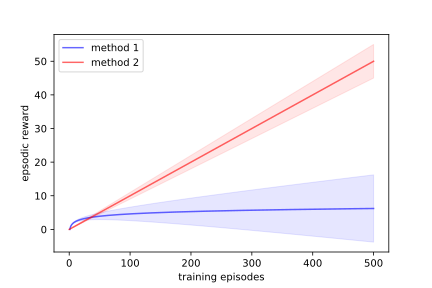
\includegraphics[width=\columnwidth]{pics/example_plot.png}
  \caption{Illustration of an figure generated using python. Make sure that all axis labels and legend texts are readable. The font size should be close to the the font size of this caption.}
  \label{fig:pythonPlotOne}
\end{figure}

Use the command \begin{verbatim} \begin{figure*}[t] ... \end{figure*} \end{verbatim} to print double column figures. 

\subsection{Tables are important}

You may want to use some online latex table generators like \url{https://www.tablesgenerator.com/}. Below are some examples. 


\begin{table}[b]
         \label{tab:exampleTableOne}
	\caption{Example table}
	\centering
	\begin{tabular}{llr}
		\toprule
		\multicolumn{2}{c}{Name} \\
		\cmidrule(r){1-2}
		First Name & Last Name & Grade \\
		\midrule
		John & Doe & $7.5$ \\
		Richard & Miles & $5$ \\
		\bottomrule
	\end{tabular}
\end{table}


\section{Conclusion}
Something about the problems of the method you used and give hints on how to solve them.

\section*{APPENDIX}

You can also directly print your source code using the command shown below.

\lstinputlisting{plot_template.py}



%----------------------------------------------------------------------------------------
%	BIBLIOGRAPHY
%----------------------------------------------------------------------------------------

\printbibliography[title={Bibliography}] % Print the bibliography, section title in curly brackets

%----------------------------------------------------------------------------------------

\end{document}
